\documentclass[handout]{beamer} % Disable pause
% \documentclass{beamer}

\usepackage{xcolor}
\definecolor{olive}{rgb}{0.3, 0.4, .1}
\definecolor{fore}{RGB}{249,242,215}
\definecolor{back}{RGB}{51,51,51}
\definecolor{title}{RGB}{255,0,90}
\definecolor{dgreen}{rgb}{0.,0.6,0.}
\definecolor{gold}{rgb}{1.,0.84,0.}
\definecolor{JungleGreen}{cmyk}{0.99,0,0.52,0}
\definecolor{BlueGreen}{cmyk}{0.85,0,0.33,0}
\definecolor{RawSienna}{cmyk}{0,0.72,1,0.45}
\definecolor{Magenta}{cmyk}{0,1,0,0}
\newcommand{\blue}[1]{\textcolor{blue}{#1}}
\newcommand{\green}[1]{\textcolor{green}{#1}}
\newcommand{\dgreen}[1]{\textcolor{dgreen}{#1}}
\newcommand{\orange}[1]{\textcolor{orange}{#1}}
\newcommand{\red}[1]{\textcolor{red}{#1}}
\newcommand{\purple}[1]{\textcolor{purple}{#1}}
\newcommand{\olive}[1]{\textcolor{olive}{#1}}

% \usepackage{beamerthemesplit} // Activate for custom appearance

\AtBeginSection[]{
  \begin{frame}
  \vfill
  \centering
  \begin{beamercolorbox}[sep=8pt,center,shadow=true,rounded=true]{title}
    \usebeamerfont{title}\insertsectionhead\par%
  \end{beamercolorbox}
  \vfill
  \end{frame}
}

\title{Introduction to Zero Knowledge Proofs}
\author{Yuncong Zhang}
\date{October 16, 2020}

\begin{document}

\frame{\titlepage}

\section[Outline]{}
\frame{\frametitle{Outline}\tableofcontents}

\section{NP Language}
\frame
{
  \frametitle{NP Language}
  \onslide<+-> What is NP language?
  \begin{itemize}
    \item<+-> Relation $\mathcal{R}=\{(x,w)\}$ is a set of instance-witness pairs
    \item<+-> Language $\mathcal{L}_\mathcal{R}=\{x:\exists w \text{ s.t.} (x,w)\in\mathcal{R}\}$ is induced from relation $\mathcal{R}$
    \item<+-> $\mathcal{L}_{\mathcal{R}}$ is in NP iff there is a \blue{deterministic polynomial time} algorithm $f$ such that $f(x,w)=1\Leftrightarrow (x,w)\in\mathcal{R}$ (we say $f$ decides $\mathcal{R}$)
  \end{itemize}
}
\frame<presentation:0>
{
  \frametitle{NP Language}
  \onslide<+-> Examples
  \begin{itemize}
    \item<+-> $\mathcal{R}=\{(x,w):w\in\mathbb{Z}\wedge x=w^2\}$\\
    $\mathcal{L}_{\mathcal{R}}=\{x:x\text{ is square integer}\}$\\
    \onslide<+-> \dgreen{We can efficiently decide $\mathcal{L}_{\mathcal{R}}$ without $w$, we say such a language is in P}
    \item<+-> $\mathcal{R}=\{(n,\text{factors}):n\in\mathbb{Z}\}$\\
    $\mathcal{L}_{\mathcal{R}}=\mathbb{Z}$
    \item<+-> $\mathcal{R}_P=\{(Q,k):Q\in\mathbb{G},k\in\mathbb{Z}_p, Q=kP\}$ \blue{$P\in\mathbb{G}$ is generator}\\
    $\mathcal{L}_{\mathcal{R}_P}=\{Q:Q\in\mathbb{G}\}$\\
    \onslide<+-> \dgreen{These languages are also in P, though sometimes it's hard to compute witness}
    \item<+-> $\mathcal{R}=\{(C,x):C\text{ is a circuit}\wedge C(x)=\mathsf{true}\}$\\
    $\mathcal{L}_{\mathcal{R}}=\{C:C\text{ is satisfiable}\}$\\
    \onslide<+-> \dgreen{This language is \textbf{NP Complete}: if there exists an efficient algorithm that decides $\mathcal{L}_{\mathcal{R}}$, then NP=P}
  \end{itemize}
}

\section{Proof Systems}
\frame
{
  \frametitle{Proof Systems}
  \onslide<+-> A proof system is an interactive protocol where the prover $\mathcal{P}$ tries to convince the verifier $\mathcal{V}$ a statement $x$ is true
  \begin{itemize}
    \item<+-> \textbf{Completeness:} if statement $x$ is true, then the verifier $\mathcal{V}$ \dgreen{accepts} (outputs 1) with probability at least $1-\eta$
    \item<+-> \textbf{Soundness:} if statement $x$ is false, then for any prover $\mathcal{P}$, the verifier $\mathcal{V}$ \red{accepts} with probability less than $\varepsilon$ (called soundness error)
  \end{itemize}
  \onslide<+-> Denote an execution of this protocol by $\langle\mathcal{P},\mathcal{V}\rangle(x)$, and $\mathsf{tr}\langle\mathcal{P},\mathcal{V}\rangle(x)$ is the \blue{transcript} of the execution, which is the collection of all interaction messages
  % \onslide<+->\begin{figure}[ht!]
  % 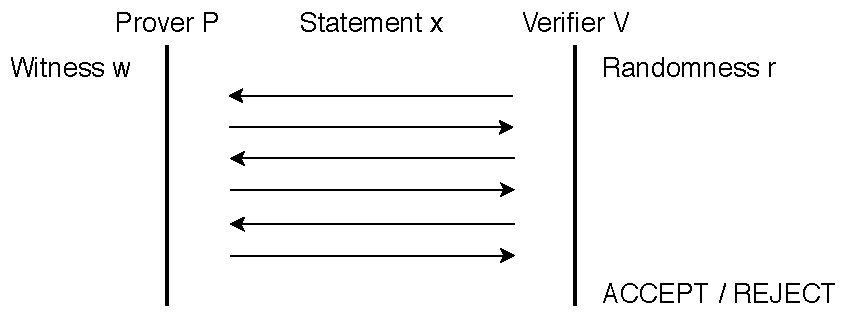
\includegraphics[width=0.8\textwidth]{images/ZKP-Proof-System.pdf}
  % \end{figure}
}

\frame
{
  \frametitle{Proof Systems}
  \onslide<+-> Examples
  \begin{itemize}
    \item<+-> For every NP language $\mathcal{L}$, the statement $x\in\mathcal{L}$ has a trivial proof system:
    \begin{enumerate}
      \item<+-> The prover sends $w$ to the verifier
      \item<+-> By definition of NP, the verifier checks $f(x,w)=1$
      \item<+-> \dgreen{Perfect completeness} and \dgreen{perfect soundness}
    \end{enumerate}
    \item<+-> Given an ECDSA public key $pk$, the prover proves that it learns the secret key $sk$
    \begin{enumerate}
      \item<+-> The verifier samples a message $m$ and sends to prover
      \item<+-> The prover generates a signature $\sigma$ and sends to verifier
      \item<+-> The verifier checks $\mathsf{ECDSAVerify(\sigma,pk,m)}=1$
    \end{enumerate}
  \end{itemize}
}

\frame
{
  \frametitle{Soundness}
  \onslide<+-> Soundness has several variations
  \begin{itemize}
    \item<+-> \textbf{Computational}: holds only for \blue{bounded} adversary
    \item<+-> \textbf{Knowledge}: requires that the prover \blue{knows} the witness
  \end{itemize}
  \onslide<+->Proof systems with different soundness have different names
  \onslide<+->\begin{table}[tb]
    \centering

    \begin{tabular}{l|cc}
    \hline

    \hline
     & \textbf{Standard} & \textbf{Knowledge} \\
    \hline
      \textbf{Statistical}   & Proof & Proof of Knowledge \\
      \textbf{Computational} & Argument & Argument of Knowledge \\
    \hline

    \hline
    \end{tabular}
  \end{table}

  \onslide<+->\begin{block}{Remark}
  Soundness is a property of the verifier.
  \end{block}
}

\frame
{
  \frametitle{Soundness}
  \onslide<+->As cryptographer, when we construct a proof system and say it has knowledge soundness, we must prove it.
  \begin{itemize}
    \item<+->But how to prove that an adversary $\mathcal{A}$ \red{knows} something?
    \item<+->Generally, we cannot prove this using game-based strategy, that means solving a hard problem when $\mathcal{A}$ \red{doesn't know}
  \end{itemize}
  \onslide<+->Instead, we use \blue{Extractor} to formalize the notion of \blue{knowing}
  \begin{itemize}
    \item<+-> Assume $\mathcal{A}$ and $\mathcal{E}$ are two algorithms, let $\mathcal{A}\|\mathcal{E}$ denote the algorithm where $\mathcal{A}$ and $\mathcal{E}$ execute simultaneously and $\mathcal{E}$ has \dgreen{white-box} access to the internal state of $\mathcal{A}$
    \item<+-> Denote by $\langle\mathcal{A}\|\mathcal{E},\mathcal{V}\rangle(x)\to(w,b)$ the protocol where $\mathcal{A}$ interacts with $\mathcal{V}$ and in the meantime $\mathcal{E}$ has access to the internal state of $\mathcal{A}$. At the end, $\mathcal{E}$ outputs $w$ and the verifier outputs $b$
  \end{itemize}
  \onslide<+->\begin{block}{Knowledge Soundness}
  For every adversary $\mathcal{A}$, there exists an extractor $\mathcal{E}_{\mathcal{A}}$, such that $\mathsf{Pr}[\langle\mathcal{A}\|\mathcal{E}_{\mathcal{A}},\mathcal{V}\rangle(x)\to(w,b):b=1\wedge (x,w)\notin\mathcal{R}]<\varepsilon$
  \end{block}
}

\frame
{
  \frametitle{Soundness}
  \onslide<+-> Another way to define the extractor
  \begin{itemize}
    \item<+->Denote by $\mathcal{E}^{\langle\mathcal{A},\mathcal{V}\rangle(x)}$ an algorithm which has \blue{black-box} access to the protocol $\langle\mathcal{A},\mathcal{V}\rangle(x)$, which means:
    \begin{itemize}
      \item $\mathcal{E}$ can read all the messages during interaction
      \item $\mathcal{E}$ can \blue{rewind} the protocol back to any point during the execution, and reexecute the protocol from that point
    \end{itemize}
  \end{itemize}
  \onslide<+->\begin{block}{Knowledge Soundness (Witness-extended emulation)}
  For every adversary $\mathcal{A}$, there exists an extractor $\mathcal{E}_{\mathcal{A}}$, such that $\mathsf{Pr}[\mathcal{E}_{\mathcal{A}}^{\langle\mathcal{A},\mathcal{V}\rangle(x)}\to w:\langle\mathcal{A},\mathcal{V}\rangle(x)\to 1 \wedge (x,w)\notin\mathcal{R}]<\varepsilon$
  \end{block}
}

\section{Zero Knowledge}
\frame
{
  \frametitle{Zero Knowledge}
  \onslide<+-> Zero-Knowledge Proofs are proof systems that also have
  \begin{itemize}
    \item<+-> \textbf{Zero-Knowledgeness:} if \dgreen{statement $x$ is true}, then the verifier \red{cannot get any information} from its view (except the correctness of $x$)
    \item<+-> The \blue{view} of the verifier consists of: \blue{randomness} $r$ and the \blue{transcript} $\mathsf{tr}\langle\mathcal{P},\mathcal{V}\rangle(x)$
  \end{itemize}
  \onslide<+-> Formally: for any verifier $\mathcal{V}$, there exists a simulator $\mathcal{S}$, which on input a \dgreen{valid statement $x$}, can sample the verifier view, i.e. the distribution of $\mathcal{S}(x)$ is \red{indifferentiable} from that of $(r,\mathsf{tr}\langle\mathcal{P},\mathcal{V}\rangle(x))$
}

\frame
{
  \frametitle{Zero Knowledge}
  \onslide<+-> ZK has several variations
  \begin{itemize}
    \item<+-> \textbf{Statistical}: statistical difference $\mathsf{SD}(\mathcal{S}(x),(r,\mathsf{tr}\langle\mathcal{P},\mathcal{V}\rangle(x)))$ is negligible (zero for perfect ZK)
    \item<+-> \textbf{Computational}: for any P.P.T. differentiator $\mathcal{D}$, $|\mathsf{Pr}[D(\mathcal{S}(x))=1]-\mathsf{Pr}[D((r,\mathsf{tr}\langle\mathcal{P},\mathcal{V}\rangle(x)))=1]|$ is negligible
    \item<+-> \textbf{Honest Verifier}: assumes that the verifier follows the protocol (but may be curious, i.e. try to learn some information from the view)
  \end{itemize}

  \onslide<+->\begin{block}{Remark}
  ZK is a property of the prover.
  \end{block}
}

\frame
{
  \frametitle{Example: Color Balls}
  \onslide<+-> Prove to a blindfold verifier that two balls have different \dgreen{colors} without revealing the colors
  \begin{enumerate}
    \item<+-> The verifier takes each ball in one hand, and shows the prover
    \item<+-> The verifier puts the hands behind its back, samples a bit $b\in\{0,1\}$ in its mind. If $b=1$, the verifier \blue{switches the balls}, otherwise it \red{does nothing}
    \item<+-> The verifier shows the balls to the prover, and the prover guesses $b'$
    \item<+-> the verifier \dgreen{accepts iff $b'=b$}
  \end{enumerate}
  \onslide<+->\textbf{Zero-knowledge}: for any verifier $\mathcal{V}$, the simulator $\mathcal{S}$ does whatever $\mathcal{V}$ does, and in the last step directly sets $b'=b$
}

\frame
{
  \frametitle{Example: Graph Isomorphism}

  \onslide<+->\begin{figure}[ht!]
  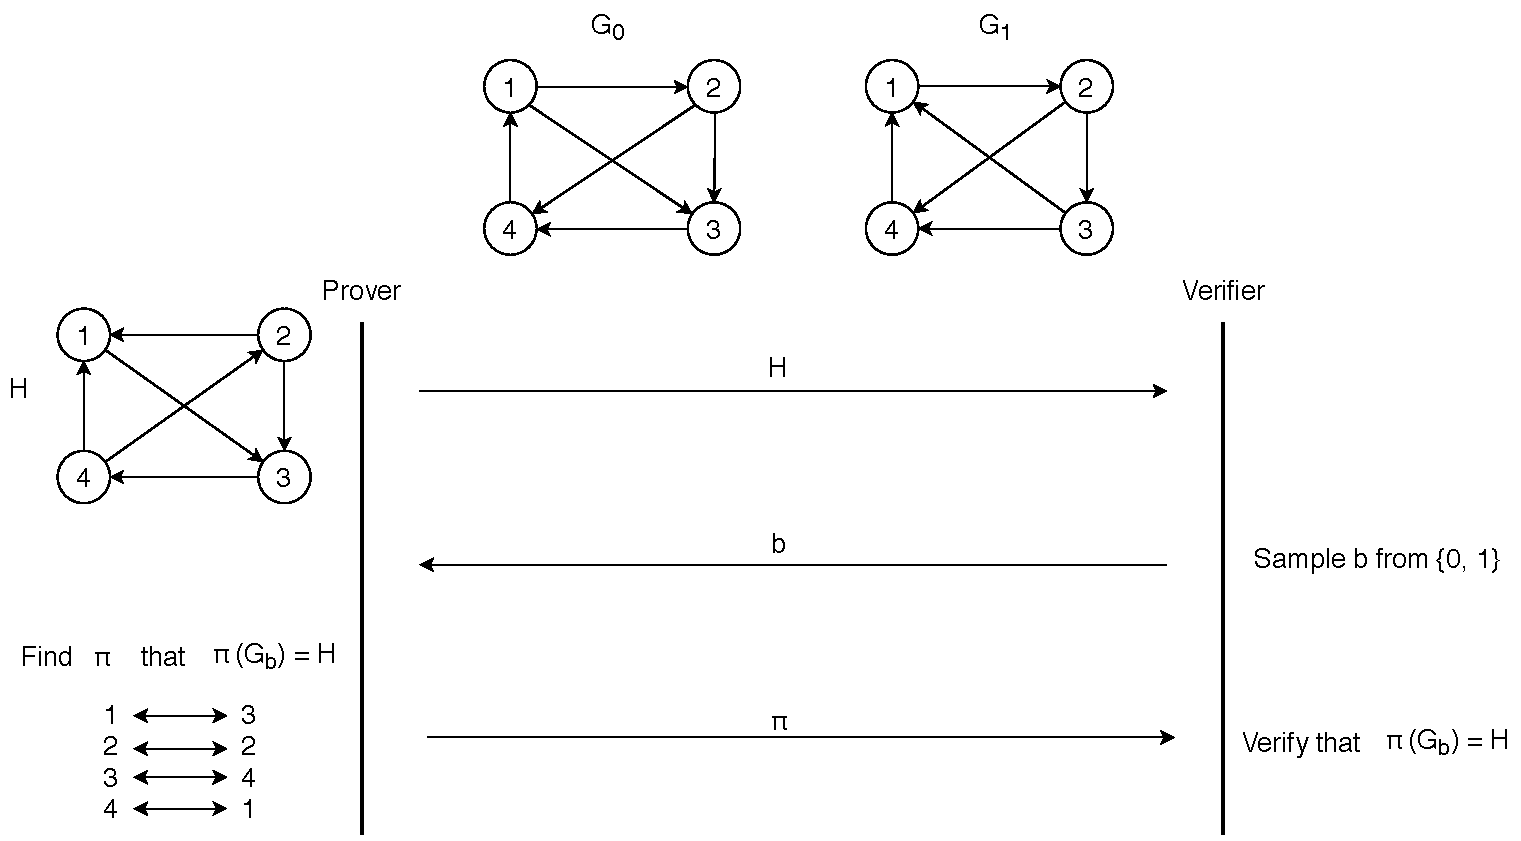
\includegraphics[width=\textwidth]{images/ZKP-Graph-Isomorphism.pdf}
  \end{figure}
  \onslide<+-> \textbf{Zero-Knowledge:} $\mathcal{S}$ samples the view $(H,b,\pi)$ as follows:
  \begin{enumerate}
    \item Uniformly sample permutation $\pi$ and bit $b$
    \item Compute $H=\pi(G_b)$, output $(H,b,\pi)$
  \end{enumerate}
}

\frame
{
  \frametitle{Example: Graph Isomorphism}
  \onslide<+->\textbf{Knowledge Soundness:} construct the following extractor $\mathcal{E}$, which has \blue{black-box} control of the protocol execution, and can read the transcript
  \begin{enumerate}
    \item<+-> $\mathcal{E}$ observes a full execution and records the transcript $(H,b,\pi_b)$
    \item<+-> $\mathcal{E}$ keeps \blue{rewinding} the execution back to the point exactly \blue{before the verifier samples $b$}, until it observes the verifier sampling \red{$b'\neq b$}
    \item<+-> $\mathcal{E}$ lets the execution proceed and obtains $(b',\pi_{b'})$
    \item<+-> $\mathcal{E}$ outputs $\pi=\pi_1^{-1}\circ\pi_0$
  \end{enumerate}
}

\frame<presentation:0>
{
  \frametitle{How can ZKP be useful?}

  \onslide<+-> The above ZKP for graph isomorphism is only useful as a toy example.
  For ZKP to be practically useful, we want
  \begin{itemize}
    \item<+-> \textbf{Non-Interactive ZK (NIZK)} so that the prover can generate a static string as the proof
    \item<+-> ZKP for general NP languages
  \end{itemize}
}

\section{NIZK}

\frame
{
  \frametitle{Non-Interactive Zero Knowledge}
  \onslide<+-> Non-interactive proof system consists of a single proof $\pi$ from prover to verifier\\\vspace{0.3cm}
  \onslide<+-> You may imagine NIZK works as follows
  \begin{itemize}
    \item<+-> $\pi\leftarrow\mathcal{P}(x,w)$
    \item<+-> $0/1\leftarrow\mathcal{V}(x,\pi)$
  \end{itemize}
  \onslide<+-> Question: does $\pi$ contain any knowledge?
  \begin{itemize}
    \item<+-> \red{Zero-knowledgeness} says \red{no}, anyone can easily generate it
    \item<+-> \blue{Soundness} says, \blue{if $x$ is hard} to decide, as a certificate to its validity, \blue{$\pi$ is also hard} to compute
  \end{itemize}
  \onslide<+-> Conclusion: NIZK only exists for easy problems.
  % \onslide<+-> However, if the \red{prover} calls the \red{simulator} to generate $\pi$, what is the result of $\mathcal{V}(x,\pi)$?
  % \begin{itemize}
    % \item<+-> If $x$ is \dgreen{true}: \blue{zero-knowledgeness} implies $\pi$ should be indistinguisbale from valid proofs, in particular, $\mathcal{V}(x,\pi)=1$ with \blue{large} probability
    % \item<+-> If $x$ is \red{false}: \blue{soundness} implies that $\mathcal{V}(x,\pi)=1$ with \blue{small} probability
  % \end{itemize}
  % \onslide<+-> In conclusion, anyone can just call $\mathcal{V}(x,\mathcal{S}(x))$ to decide $x$.\\\vspace{0.3cm}
  % \onslide<+-> Threfore, NIZK only exists for trivial problems.
}


\frame
{
  \frametitle{Non-Interactive Zero Knowledge}
  \onslide<+-> NIZK is only possible in \blue{Common Reference String (CRS)} model
  \begin{itemize}
    \item<+-> Structured Reference String (SRS)
    \item<+-> Uniform Random String (URS)
  \end{itemize}
  \onslide<+-> Additionally, we need at least one of
  \begin{itemize}
    \item<+-> Random Oracle (RO) model
    \item<+-> Trusted Third Party (TTP)
  \end{itemize}

  % \onslide<+->\begin{table}[tb]
  %   \centering
%
  %   \begin{tabular}{l|cc}
  %   \hline
%
  %   \hline
  %                  & \textbf{URS} & \textbf{SRS} \\
  %   \hline
  %     \textbf{RO}  & $\checkmark$ & $\checkmark$ \\
  %   \hline
  %     \textbf{TTP} & $\times$            & $\checkmark$ \\
  %   \hline
  %   \end{tabular}
  % \end{table}
}

\frame<presentation:0>
{
  \frametitle{From ZKP to NIZK}

  \onslide<+-> The idea behind NIZK is running the verifier ``in the prover's mind''

  \begin{itemize}
    \item<+-> The key is to simulate the verifier messages \textbf{unpredictably}
    \item<+-> Random Oracle model: simulate the verifier message with Random Oracle outputs, where the input is all the prover messages so far
    \item<+-> Common Reference String model: generate the verifier messages in advance, and hide them inside CRS
  \end{itemize}
}

% \section{ZKP for General NP}

\frame<presentation:0>
{
  \frametitle{Does ZKP exist for general NP languages?}
  \begin{itemize}
    \item<+-> Short answer: YES. But ...
    \item<+-> We need some cryptography
    \begin{itemize}
      \item<+-> Specifically, we need to assume that One-Way-Function exists
    \end{itemize}
    \item<+-> We also need to lower the security requirement, in either or both of the following aspects
    \begin{itemize}
      \item<+-> \textbf{Computational Zero-Knowledge}: the sampled verifier view is only computationally indifferentiable from the real view
      \item<+-> \textbf{Computational Soundness}: the soundness security only holds against computationally bounded prover
    \end{itemize}
  \end{itemize}
  \onslide<+->\begin{block}{Remark}
  Strictly speaking, proof systems with only computational soundness are no longer proof systems, but argument systems
  \end{block}
}

\frame<presentation:0>
{
  \frametitle{How to construct ZKP for general NP languages?}

  \onslide<+-> It suffices to construct a ZKP for any NP-Complete language, e.g. 3-SAT, Graph-3-Color. However
  \begin{itemize}
    \item<+-> It is not efficient to transform general NP languages to 3-SAT or Graph-3-Color in practice
  \end{itemize}
  \onslide<+-> Usually, we only choose from the \textbf{Circuit-Satisfiability (CSAT)} languages.
  \begin{itemize}
    \item BCSAT: Boolean circuit satisfiability, the circuit deals with 0-1 values, and consists of boolean gates like AND, OR, NOT, XOR
    \item ACSAT: Arithmetic circuit satisfiability, the circuit deals with finite field $\mathbb{F}$, consists of addition gates and multiplication gates
  \end{itemize}
}

\frame<presentation:0>
{
  \frametitle{What is CSAT problem?}

  \onslide<+-> Given a circuit $C$, with $m$ input wires and 1 output wire
  \begin{itemize}
    \item<+-> An instance $x$ of CSAT is an assignment to the first $n$ inputs
    \item<+-> The CSAT problem is, given the first $n$ inputs, decides if there is an assignment of the rest $m-n$ inputs, such that the circuit $C$ outputs 1
    \item<+-> By programming $C$, the CSAT problem can encode any NP problem
  \end{itemize}

  \onslide<1->\begin{figure}[ht!]
  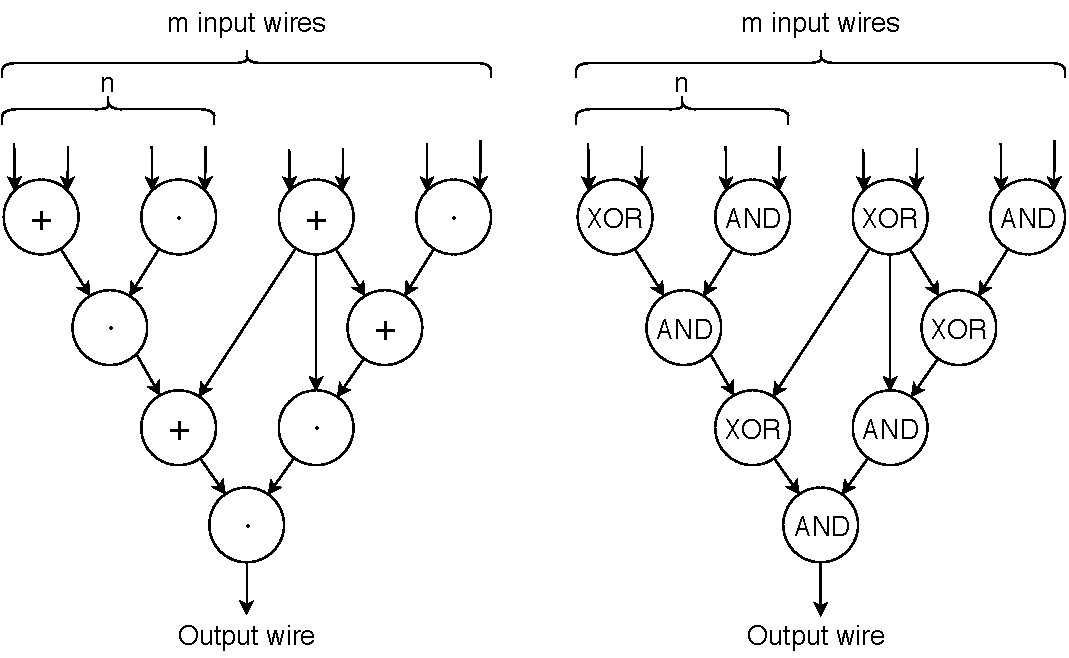
\includegraphics[width=0.6\textwidth]{images/ZKP-Circuits.pdf}
  \end{figure}
}

\frame<presentation:0>
{
  \frametitle{How to construct ZKP for CSAT?}

  \onslide<+-> There are many branches of research
  \begin{itemize}
    \item<+-> Pairing-based: most efficient, but requires trusted setup, and relies on elliptic curves that support pairing
    \item<+-> PCP-based: PCP is a more powerful proof model than interactive proofs, and can be compiled to interactive arguments using cryptography
    \item<+-> GKR-based: GKR is an interactive protocol for uniform circuits
    \item<+-> MPC-based: use MPC-in-the-head framework, directly apply techniques from MPC
  \end{itemize}
}

\frame
{
  \center\huge Q/A
}

\end{document}
